%\motto{Use the template \emph{chapter.tex} to style the various elements of your chapter content.}
\chapter{Medizinische Anwendungsgebiete}
\label{trends} % Always give a unique label
% use \chaptermark{}
% to alter or adjust the chapter heading in the running head

\chapterauthor{Martin Maier, Siri Wandel}

\abstract{some abstract}

\section{Relevanz \& Problemstellung}


\section{Top 3 Anwendungsfelder (Praxis \& Theorie)}
\label{med:applicationFields}
Die potenziellen Einsatzmöglichkeiten von Quantencomputern im Gesundheitswesen sind vielfältig, wie Abbildung \ref{fig:use-cases-medicine} verdeutlicht. Sie reichen von molekularer Simulation über Krebsbehandlung bis hin zu Bildanalyseverfahren. In diesem Abschnitt liegt der Fokus auf den drei Anwendungsfeldern, die aktuell sowohl in der Forschung als auch in der industriellen Entwicklung eine herausragende Rolle spielen: Wirkstoffentwicklung, Proteinstrukturvorhersage und Personalisierte Medizin.\\
\\
\begin{figure}[ht]
    \centering
    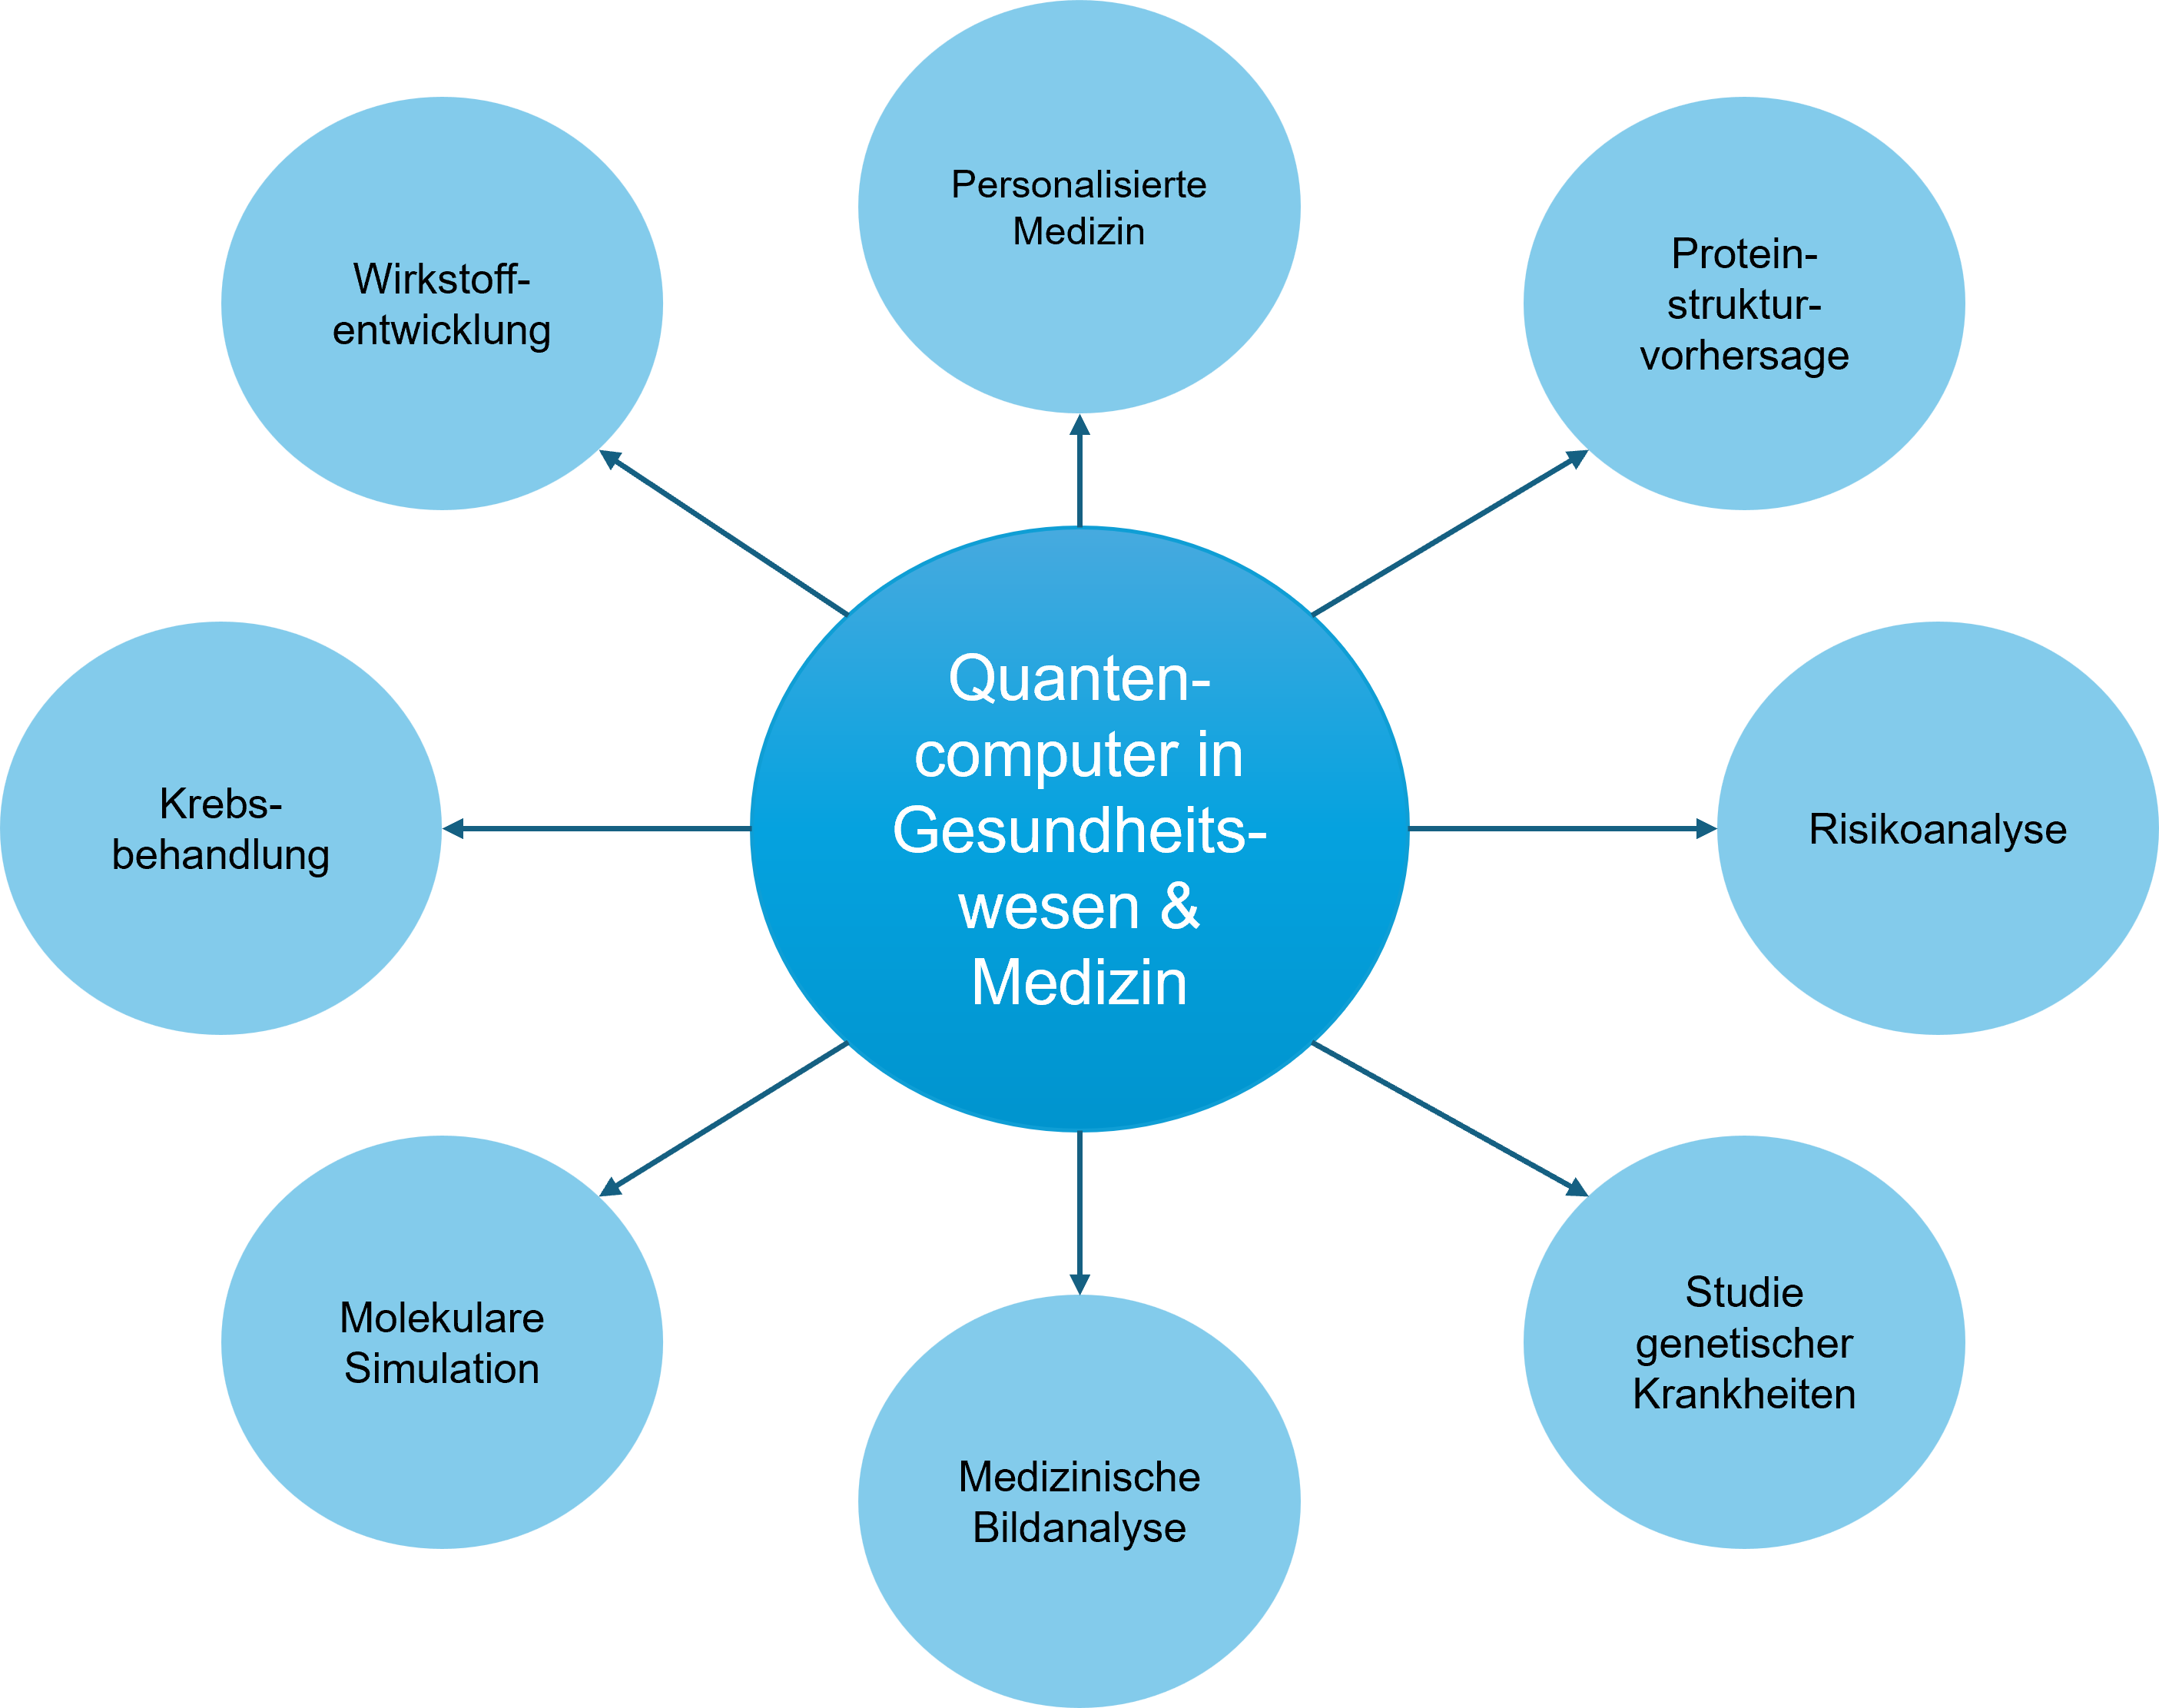
\includegraphics[width=.8\textwidth]{images/medicine/AnwendungsfelderMedizin.png}
    \caption{Übersicht möglicher Einsatzfelder von Quantencomputern in der Medizin. (Eigene Darstellung nach \cite{dhande_quantum_2023}.)}
    \label{fig:use-cases-medicine}
\end{figure}
\\
Diese Auswahl basiert auf drei qualitativen Kriterien: Erstens adressieren diese Bereiche relevante medizinische Herausforderungen. Zweitens zeichnen sie sich durch eine besonders hohe rechnerische Komplexität aus, die den Einsatz von Quantencomputern sinnvoll erscheinen lässt. Drittens bestehen bereits erste praxisnahe Anwendungen und Pilotprojekte, die eine Brücke zwischen theoretischem Potenzial und konkreter Nutzung bilden. Die Auswahl orientiert sich somit nicht nur an theoretischem Potenzial, sondern auch an praktischer Umsetzbarkeit und gesellschaftlicher Relevanz.

\subsection{Wirkstoffentwicklung}
Die Entwicklung neuer Wirkstoffe ist grundlegend mit hohen Kosten verbunden. Das liegt besonders an langen Entwicklungszyklen und einer geringen Erfolgsquote. Der Einsatz von Computern, besonders im Rahmen des Computer"=Aided Drug Design (CADD), ist in der pharmazeutischen Forschung etabliert. Dies stößt jedoch bei der Modellierung komplexer molekularer Systeme an seine Grenzen (Vgl. \cite{bertl_quantum_2025}).

\subsubsection*{Compound Screening \& Lead"=Optimierung}
Quantencomputer versprechen, diese Prozesse durch genauere und schnellere Simulationen von Molekülen und deren Wechselwirkungen erheblich zu verbessern. Dabei konzentrieren sich aktuelle Quantencomputing"=Anwendungen in der pharmazeutischen Forschung besonders auf zwei frühe Phasen der Wirkstoffentwicklung: das \textit{Compound Screening} und die \textit{Lead"=Optimierung}. Beim Compound Screening werden sehr viele verschiedene chemische Verbindungen daraufhin untersucht, ob sie grundsätzlich an ein Zielmolekül (z.B. ein krankheitsrelevantes Protein) binden können. In der Lead"=Optimierung werden dann vielversprechende Kandidaten gezielt verbessert, um deren Wirksamkeit und Verträglichkeit zu steigern. Quantencomputer können in diesen Phasen helfen, indem sie Wechselwirkungen zwischen Molekülen genauer simulieren und energetisch günstige Strukturen besser vorhersagen (Vgl. \cite{zinner_quantum_2021}).

\subsubsection*{Quantenchemische Simulation}
Auf theoretischer Ebene gilt die quantenchemische Berechnung von Molekül"=Energien als eines der vielversprechendsten Anwendungsfelder des Quantencomputings. Sie ist essenziell für die Ermittlung von Bindungsaffinitäten, Reaktionspfaden und energetisch bevorzugten Konformationen, welche zentrale Größen in der computergestützten Wirkstoffentwicklung sind. Wie \cite{cao_quantum_2019} betonen: Das klassische Problem, dessen Lösung vom Quantencomputing erwartet wird, ist die Berechnung von Grundzustands- und angeregten Zustandsenergien kleiner Moleküle. Solche Berechnungen dienen als Ausgangspunkt für die Bestimmung vieler nützlicher Größen, wie etwa Reaktionspfaden, Bindungsenergien und Reaktionsgeschwindigkeiten chemischer Prozesse. (eigene Übersetzung nach \cite{cao_quantum_2019}.) Zentral ist demnach die Berechnung von Molekülenergien, da sie viele wichtige chemische Eigenschaften bestimmt.

\subsubsection*{Virtuelles Screening und datengetriebene Modellierung}
Beim \textit{virtuellen Screening} handelt es sich um einen frühen Schritt im Prozess der Wirkstoffentwicklung. Dabei werden mit Hilfe von Computern große Datenbanken nach Molekülen durchsucht, die an ein bestimmtes krankheitsrelevantes Ziel binden könnten. So lassen sich vielversprechende Wirkstoffkandidaten schneller finden und unnötige Labortests vermeiden. Klassische Methoden stoßen dabei aber oft an Grenzen: Die Modelle sind manchmal ungenau, liefern viele falsche Treffer und brauchen viel Rechenleistung. Neue Ansätze wie Quantum Machine Learning (siehe Kapitel \ref{alg:qml}) können hier helfen. Mit Quantencomputern lassen sich Molekülwechselwirkungen genauer simulieren und komplexe Daten effizienter verarbeiten. Techniken wie Quanten"=Neuronale Netzwerke, Quanten"=Kernel oder spezielle Quanten"=Suchalgorithmen ermöglichen ein gezielteres und schnelleres Screening. (Vgl. \cite{kumar2024})


\subsection{Proteinstrukturvorhersage}
\label{med:protein}
Die bisher etablierten Methoden zur Proteinstrukturvorhersage haben bereits beeindruckende Fortschritte erzielt. Mit experimentellen Ansätzen sowie durch KI"=basierte Modelle wie AlphaFold, RoseTTaFold und verwandte Systeme lassen sich für viele Proteine dreidimensionale Strukturen bereits mit hoher Genauigkeit vorhersagen. (Vgl. \cite{jumper2021, baek2021})

\subsubsection*{Grenzen klassischer Methoden}
Diese klassischen Methoden basieren meist auf Mustern aus bekannten Proteinstrukturen und liefern häufig nur ein begrenztes Verständnis der physikalischen Prozesse, die der Proteinfaltung zugrunde liegen. Das erschwert insbesondere die Vorhersage bei synthetischen oder stark abweichenden Aminosäuresequenzen. Studien zeigen, dass Modelle wie AlphaFold2 bei solchen Sequenzen außerhalb ihres Trainingsdatensatzes unzuverlässige Ergebnisse liefern können (Vgl. \cite{outeiral2022}). Physikbasierte Verfahren wie die Molekulardynamik bieten zwar grundsätzlich eine höhere Genauigkeit, sind jedoch für größere Proteine extrem rechenintensiv und in der Praxis kaum skalierbar (Vgl. \cite{doga_perspective_2024}). Diese Einschränkungen verdeutlichen den Bedarf an alternativen Modellierungsansätzen.

\subsubsection*{Quantenbasierte Faltungsmodelle}
Quantencomputer könnten eine vielversprechende Alternative bieten, da sie durch Quantenparallelismus potenziell viele Faltungszustände gleichzeitig analysieren können (Vgl. \cite{doga_perspective_2024}). Aktuelle Forschungsarbeiten formulieren die Proteinfaltung dabei als Optimierungsproblem und setzen auf Quantenalgorithmen sowie vereinfachte physikalische Modelle. Zwei Ansätze haben sich dabei als besonders vielversprechend erwiesen: Hybridverfahren mit VQE und quantenbasierte Gittermodelle.\\
\\
Im Ansatz von \citeauthor{doga_perspective_2024} wurde ein hybrider Algorithmus eingesetzt, der klassische Optimierung mit einem VQE kombiniert. Ziel war die Vorhersage der Struktur eines kurzen Abschnitts mit sieben Aminosäuren aus dem Helikaseprotein des Zika"=Virus. Solche Abschnitte werden als Loops bezeichnet. Sie verbinden regelmäßige Strukturelemente wie Alpha"=Helices und Beta"=Faltblätter und sind häufig entscheidend für die Funktion eines Proteins. Die räumliche Anordnung der Atome in diesem Abschnitt, also die sogenannte Konformation, wurde anschließend mit bekannten Referenzdaten verglichen. Die mittels Quantencomputer berechnete Struktur wich deutlich weniger vom experimentell bestimmten Referenzmodell ab als die Vorhersage von AlphaFold2. Der mittlere Abstand der Atome (RMSD) betrug etwa 1,88 Å bei der Quantenmethode und 3,53 Å bei AlphaFold2. Das zeigt, dass quantenbasierte Verfahren bereits heute genauere Ergebnisse liefern können als etablierte KI"=Modelle. Zumindest für kleinere, aber strukturell anspruchsvolle Proteinbereiche. (Vgl. \cite{doga_perspective_2024})\\
\\
Ein weiterer Ansatz basiert auf Gittermodellen. \citeauthor{robert_resource-efficient_2021} verwendeten ein solches Modell zur Faltung kurzer Peptide mit IBM-Quantenhardware. Ein 10"=Aminosäure"=Peptid (Angiotensin) wurde auf 22 Qubits, ein 7-Aminosäure-Peptid auf 9 Qubits kodiert. Die Ergebnisse zeigen, dass selbst kleine Quantencomputer bereits in der Lage sind, realistische Faltungskonfigurationen effizient zu berechnen. (Vgl. \cite{robert_resource-efficient_2021})


\subsection{Personalisierte Medizin}
Die personalisierte Medizin verfolgt das Ziel, medizinische Entscheidungen stärker an den individuellen Eigenschaften eines Patienten auszurichten, etwa an genetischen Merkmalen, Krankheitsverläufen oder Therapieansprechen. Das bedeutet, dass aus komplexen, oft hochdimensionalen Daten wie Genomsequenzen, Laborwerten oder Bilddaten präzise Vorhersagen abzuleiten sind. Klassische Methoden stoßen hierbei zunehmend an ihre Grenzen, insbesondere bei kleinen Datensätzen, hoher Variabilität oder stark nichtlinearen Zusammenhängen. Auch maschinelles Lernen stoßt bei individuellen oder seltenen Fällen oft an seine Grenzen. Bei wenigen Trainingsdaten führen sie zu unsicheren Diagnosen und Therapieentscheidungen. (Vgl. \cite{gupta_systematic_2025}).

\subsubsection*{P5"=Medizin}
In der aktuellen Forschung wird personalisierte Medizin zunehmend als sogenanntes P5"=Modell verstanden. Dieses erweitert das bisherige P4"=Modell um eine fünfte Dimension: \textit{psychokognitiv}. Die fünf Elemente lauten: vorhersagend (predictive), vorbeugend (preventive), personalisiert, beteiligend (participatory) und psychokognitiv. Letztere betont psychologische und kognitive Faktoren wie Werte, Lebensqualität und Gesundheitskompetenz. Diese beeinflussen, wie Patienten mit Erkrankungen umgehen und wie sie auf Therapien reagieren. (Vgl. \cite{gorini_p5_2011})\\
\\
Quantencomputing kann in diesem Kontext neue Wege eröffnen. Durch seine Fähigkeit, viele Datenmuster gleichzeitig zu analysieren, lassen sich verhaltensbezogene Einflussfaktoren stärker in personalisierte Modelle integrieren. Besonders vielversprechend ist hier der Einsatz von Quantum Machine Learning, also von Modellen, die klassische Lernverfahren mit quantenmechanischen Elementen kombinieren (Vgl. \cite{bertl_quantum_2025}.)

\subsubsection*{Frühe Anwendungen von Quantum Machine Learning}
Eine aktuelle Übersichtsarbeit zeigt, dass sich erste klinisch relevante QML-Anwendungen zum Beispiel in der EKG"=Analyse, Genomik oder Bildgebung bereits auf echter Quantenhardware testen lassen, wenn auch bisher in begrenztem Umfang (Vgl. \cite{gupta_systematic_2025}). Besonders Genomik und Bildgebung ermöglichen eine präzisere Diagnostik und auf individuelle genetische Profile abgestimmte Therapieansätze.\\
\\
Ein konkretes Beispiel liefert eine Studie zur Vorhersage von Arzneimittelwirkungen bei Krebspatienten. In dieser erzielt ein hybrides QNN eine bis zu 15 Prozent höhere Genauigkeit als klassische Modelle, bei signifikant kürzerer Trainingszeit (Vgl. \cite{sagingalieva_hybrid_2023}).\\
\\
\begin{table}[ht]
\centering
\renewcommand{\arraystretch}{1.3}
\resizebox{\textwidth}{!}{
\begin{tabular}{|p{2.3cm}|p{4.5cm}|p{2.5cm}|p{4.5cm}|}
\hline
\textbf{Anwendungsfeld} & \textbf{Rechnerische Herausforderung} & \textbf{Quantenansatz / Algorithmus} & \textbf{Warum QC relevant?} \\
\hline
Drug Discovery & Molekül-Energieberechnung, Bindungsaffinitäten & VQE, QPE & Klassische Methoden zu ungenau oder zu langsam \\
\hline
Proteinstruktur & Kombinatorische Explosion möglicher Faltungen & QAOA, Hybridalgorithmen & QC kann Zustände simultan analysieren \\
\hline
Personalisierte Medizin & Mustererkennung in hochdimensionalen Daten & QML, QNN & Klassische Modelle überfordert bei komplexer Nichtlinearität \\
\hline
\end{tabular}
}
\caption{Anwendungsfelder des Quantencomputings in der Medizin und Pharmazie}
\label{tab:qc_medizin}
\end{table}
\\


\section{Top Technologien \& Algorithmen}

\subsection{Variational Quantum Eigensolver (VQE)}
Der Variational Quantum Eigensolver (VQE) ist ein Algorithmus zur Lösung quantenchemischer Probleme und findet zunehmend Anwendung im medizinischen Kontext. In der quantenchemischen Simulation kann VQE genutzt werden, um Molekülenergien, Bindungsaffinitäten und Reaktionspfade zu berechnen. Diese Größen sind entscheidend für die Beurteilung chemischer Stabilität und Reaktivität und spielen eine wichtige Rolle bei der frühen Identifikation potenzieller Wirkstoffe (Vgl. \cite{palFuturePotentialQuantum2024}; \cite{cao_quantum_2019}). Darüber hinaus wird VQE auch in der Strukturbiologie erforscht. Er kann eingesetzt werden, um die Energie von Proteinbausteinen oder Ligand-Protein-Komplexen abzuschätzen, was dazu beiträgt, molekulare Wechselwirkungen besser zu verstehen (\cite{marchettiQuantumComputingAlgorithms2022}). Studien deuten zudem darauf hin, dass VQE künftig auch für die Simulation individueller Stoffwechselprozesse genutzt werden könnte. Dies betrifft beispielsweise Anwendungen in der personalisierten Medizin, etwa zur Vorhersage individueller Therapieerfolge oder bei der Entwicklung neuer Kontrastmittel für bildgebende Verfahren (\cite{palFuturePotentialQuantum2024}).

\subsection{Quantum Phase Estimation (QPE)}
Der Quantum Phase Estimation (QPE) Algorithmus gilt als zentrale Methode zur präzisen Bestimmung von Grundzustandsenergien von Molekülen und ist damit von besonderem Interesse für die Wirkstoffentwicklung, etwa bei pharmazeutisch relevanten Substanzen wie Ibrutinib. Im Vergleich zu klassischen Verfahren bietet QPE das Potenzial für eine exponentielle Beschleunigung solcher Berechnungen. Die herkömmliche Lehrbuchvariante von QPE ist jedoch sehr ressourcenintensiv und anfällig für Fehler, da sie zahlreiche Hilfs-Qubits und tiefe Schaltkreise erfordert. Um diese Limitierungen zu überwinden, wurden speziell für frühe fehlertolerante Quantencomputer (EFTQCs) optimierte Protokolle wie Iterative Phase Estimation (IPE), Robust Phase Estimation (RPE), Quantum Complex Exponential Least Squares (QCELS) und Multi"=Modal Multi"=Level QCELS (MMQCELS) entwickelt. Diese reduzieren sowohl die Zahl der benötigten Ancilla"=Qubits als auch die Schaltungstiefe und verbessern die Robustheit gegenüber Fehlern deutlich. Studien zeigen, dass das Berechnungsvolumen im Vergleich zur klassischen QPE um ein Vielfaches gesenkt werden kann. Teilweise um das bis zu 300-Fache. Ergänzend leisten Fortschritte in der Optimierung der Simulationstechniken und der Fehlerminderung einen Beitrag zur praktischen Umsetzbarkeit dieser Methoden. (Vgl. \cite{nelson_assessment_2024}; \cite{blunt_perspective_2022}; \cite{blunt_statistical_2023})

\subsection{Quantum Approximate Optimization Algorithm (QAOA)}
QAOA ist ein variationaler Quantenalgorithmus zur näherungsweisen Lösung kombinatorischer Optimierungsprobleme, der im medizinischen Bereich insbesondere in der Proteinfaltung und im molekularen Docking Anwendung findet. Für das Proteinfaltungsproblem wurde QAOA in vereinfachten Gittermodellen getestet, wobei es energiearme Konformationen mit höherer Wahrscheinlichkeit erzeugen konnte als rein zufälliges Sampling. Allerdings erfordern realistischere Modelle deutlich tiefere Quantenschaltkreise, was eine Anwendung auf atomarer Ebene derzeit noch erschwert. Größeres Potenzial zeigt QAOA im Bereich des molekularen Dockings, das für die Entwicklung neuer Medikamente zentral ist. Durch die Formulierung des Problems als maximal gewichtete Clique lassen sich mit dem verbesserten DC"=QAOA"=Ansatz biologisch relevante Bindungsstellen effizienter identifizieren. Fallstudien mit relevanten Zielproteinen wie SARS"=CoV"=2 Mpro, DPP-4 und HIV-1 gp120 belegen eine hohe Übereinstimmung mit bekannten Strukturen. Gleichzeitig zeigt DC"=QAOA Vorteile bei der Ressourcennutzung, da es weniger Gatter und Iterationen benötigt als klassische Varianten. Herausforderungen bestehen weiterhin in der Stabilität der Optimierung, insbesondere bei komplexeren molekularen Systemen. (Vgl. \cite{DingMolecularDocking2024}; \cite{boulebnane_peptide_2023})

\subsection{Hybride Quantenklassische Algorithmen}
Hybride quantenklassische Algorithmen kombinieren klassische Rechenmethoden mit quantenmechanischen Komponenten und gelten als vielversprechender Ansatz für medizinische Anwendungen im Zeitalter begrenzter Quantenhardware. Besonders in der personalisierten Medizin und Wirkstoffentwicklung zeigen sich erste sinnvolle Einsatzmöglichkeiten. So lassen sich etwa Biomarker für bestimmte Krebsarten wie das klarzellige Nierenzellkarzinom genauer klassifizieren, was die Diagnose verbessern und Therapien gezielter ermöglichen kann. Auch in der computergestützten Entwicklung neuer Medikamente bieten hybride Verfahren Vorteile, zum Beispiel bei der Simulation chemischer Bindungen oder der Bewertung pharmakologisch relevanter Energieprofile. Diese Ansätze verdeutlichen, dass sich Quantencomputing bereits heute sinnvoll mit bestehenden Methoden verknüpfen lässt, um medizinische Entscheidungsprozesse zu unterstützen. (Vgl. \cite{li_hybrid_2024}; \cite{Astuti2025})

\subsection{Quantum Machine Learning (QML) \& Quantum Neural Networks (QNN)}
Quanten-Maschinelles Lernen (QML) und Quanten-Neuronale Netzwerke (QNN) sind speziell entwickelte Quantenalgorithmen zur Analyse klassischer Gesundheitsdaten. Insbesondere im Zuge der zunehmenden Digitalisierung, etwa durch elektronische Gesundheitsakten, gelten sie als vielversprechende Werkzeuge für klinische Entscheidungshilfen, Gesundheitsprognosen und kontinuierliches Monitoring. QNNs kommen dabei als gate-basierte Modelle zum Einsatz, die sich gezielt für solche Aufgaben einsetzen lassen. Eine systematische Übersichtsarbeit zu Veröffentlichungen zwischen 2015 und 2024 zeigt jedoch, dass es bislang an empirischer Evidenz für einen klaren Vorteil gegenüber klassischen Verfahren mangelt. Die meisten Studien konzentrierten sich auf Diagnose- und Prognoseanwendungen, während wichtige Bereiche wie Public Health oder Versorgungsforschung kaum berücksichtigt wurden. Darüber hinaus erfolgten viele Untersuchungen unter idealisierten Bedingungen und setzten vereinfachte, lineare Modelle ein, ohne reale Fehlerquellen zu integrieren. (Vgl. \cite{gupta_systematic_2025}

\subsection{Technologische Frameworks}
Die in diesem Abschnitt vorgestellten technologischen Frameworks orientieren sich an den in Kapitel \ref{med:applicationFields} beschriebenen Anwendungsfeldern. Ziel ist es, die eingesetzten Softwarestacks und Entwicklungstools entlang ihrer praktischen Einsatzbereiche in der Wirkstoffentwicklung, der Proteinstrukturvorhersage und der personalisierten Medizin systematisch darzustellen. Auf diese Weise wird deutlich, wie spezifische Quantenalgorithmen in den jeweiligen medizinischen Kontexten technologisch implementiert werden.\\

\subsubsection*{Wirkstoffentwicklung}
Die praktische Umsetzung der Quantenalgorithmen für medizinische Anwendungen erfordert leistungsfähige Software"=Stacks, die Quanten-Hardware und klassische Algorithmen verbinden. Für die Wirkstoffentwicklung werden vor allem Frameworks genutzt, die komplexe \textit{Molekül"=Hamilton"=Operatoren} bearbeiten und Verfahren wie VQE oder QPE effizient implementieren. Bei den Operatoren handelt es sich um mathematische Ausdrücke, die alle relevanten physikalischen Eigenschaften eines Moleküls quantenmechanisch beschreiben. Der Hamilton"=Operator bildet somit die Grundlage für die Simulation von Molekülzuständen, da er die Energieverteilung eines Systems vollständig bestimmt (Vgl. \cite{mcardle}).\\

So bietet IBM Qiskit mit dem Qiskit Nature"=Modul spezialisierte Werkzeuge zur Darstellung chemischer Systeme und zum Lösen von Grundzustandsproblemen in Molekülen. (Vgl. \cite{noauthor_qiskit_2022})\\

Microsofts Q\# Quantum Development Kit (QDK) enthält ebenfalls eine Chemie-Bibliothek mit qubitisierten Fermionen-Operatoren sowie Implementierungen von Hamilton-Simulatoren (Trotterisierung, Qubitierung). (Vgl. \cite{msazure}) \\

Amazon Braket ist ein vollständig verwalteter Cloud-Dienst von AWS, der es Forscherinnen und Forschern ermöglicht, Quantenalgorithmen zu entwerfen, auf verschiedenen Simulatoren zu testen und auf realen Quantencomputern auszuführen. Damit bietet Braket eine flexible Entwicklungsumgebung für hybride quantenklassische Workflows in der Arzneimittelforschung. Besonders relevant für medizinische Anwendungen ist der Zugriff auf unterschiedliche Hardwareplattformen innerhalb eines einheitlichen SDK. Braket unterstützt unter anderem gatterbasierte Quantencomputer von IonQ, IQM und Rigetti sowie einen Analog Hamiltonian Simulator (AHS) von QuEra. Letzterer erlaubt die direkte Simulation physikalischer Systeme auf Basis kontinuierlicher Hamilton-Operatoren, was für bestimmte molekulare Strukturberechnungen von Vorteil sein kann. (Vgl. \cite{amazonbraket})\\

Dieser flexible Ansatz wird beispielsweise im AWS"=Toolkit QCEDD genutzt, das eingebaute Beispiele für Aufgaben wie molekulares Docking und Faltungsprobleme in der Wirkstoffforschung enthält. (Vgl. \cite{amazonscience})\\ %evtl. git repo zitieren

%besonders beim virtuellen screening relevant 

\subsubsection*{Proteinstrukturvorhersage}
Die Vorhersage von Proteinstrukturen ist ein hochdimensionales Optimierungsproblem. Klassischerweise modelliert man Proteine auf Gitternetzen, um die Konformationsräume lösbar zu machen. Wie bereits in Kapitel \ref{med:protein} dargelegt, sind Quantenoptimierungsalgorithmen wie QAOA dafür gut geeignet. (Vgl. \cite{boulebnane})\\

Zur praktischen Umsetzung von Algorithmen wie QAOA in der Proteinstrukturvorhersage wird geeignete Software benötigt, die die Komplexität quantenmechanischer Optimierung handhabbar macht. Ein bekanntes Framework in diesem Bereich ist \textit{PennyLane}. Es ist eine plattformunabhängige Open"=Source"=Bibliothek für Quantencomputing und Quantum Machine Learning, die für wissenschaftliche Anwendungen entwickelt wurde. Durch PennyLane können Quantenalgorithmen mit klassischen Lernverfahren kombiniert werden. Das ist besonders bei der Proteinstrukturvorhersage von Vorteil, da hier sowohl quantenbasierte Optimierung, als auch klassische Auswertungsverfahren erforderlich sind. (Vgl. \cite{PennyLane})\\

Das Start"=up Menten AI nutzt PennyLane für die Entwicklung neuer proteinbasierter Wirkstoffe. Ziel ist es, Quantencomputing und klassische Verfahren so zu kombinieren, dass neue Wirkstoffkandidaten schneller und gezielter gefunden werden können. Dabei setzt Menten AI auf PennyLane, um Quantenalgorithmen effizient einzubinden und bioaktive Peptide für neue Therapien zu entwickeln. Das heißt, sie nutzen die Software, um schneller passende Wirkstoffe zu finden, die gut an bestimmte Krankheitsziele andocken können. (Vgl. \cite{xanadu2022})\\



\subsubsection*{Personalisierte Medizin}
In der personalisierten Medizin stehen große, hochdimensionale Datensätze (Genomik, Bildgebung, EKG, klinische Parameter) im Mittelpunkt. Hier kommen Frameworks zum Einsatz, die Quantenmodelle in klassische Machine"=Learning"=Pipelines einbetten. Ein Beispiel ist die Kombination aus \textit{Cirq} und \textit{TensorFlow Quantum}. Damit lassen sich Quantenalgorithmen direkt in klassische Lernmodelle integrieren. So entstehen hybride neuronale Netze, die klassische und quantenbasierte Rechenschritte verbinden. Das hilft dabei, komplexe medizinische Daten genauer auszuwerten und Muster zu erkennen, die für individuelle Behandlungsentscheidungen wichtig sind. (Vgl. \cite{tensorflowQuantum2020})

\section{Wichtige Unternehmen \& Akteure}
Im Zuge des zunehmenden Interesses an der Nutzung von Quantencomputern zur Lösung komplexer Probleme in der Medizin- und Pharmaforschung etablieren sich weltweit führende Technologieunternehmen, Start-ups sowie Forschungs- und Bildungseinrichtungen als zentrale Akteure, die entsprechende Ressourcen bereitstellen und wissenschaftliche Kooperationen eingehen. 
Der folgende Abschnitt stellt eine Auswahl einiger der wichtigsten Unternehmen und Akteure dar, die mit Hardware- und Softwarelösungen sowie durch wissenschaftliche Expertise zur Beschleunigung medizinischer Forschungsprozesse mithilfe von Quantentechnologie beitragen.\\

IBM Quantum gehört zu den Vorreitern auf dem Gebiet und stellt vielfältige Hardware- und Softwareressourcen bereit, die das Lernen, Experimentieren und die Zusammenarbeit in dem Bereich des Quantencomputings fördern.(Vgl. \cite{abughanemIBMQuantumComputers2025}) 
Seit der Einführung des ersten cloudbasierten Quantencomputers im Jahr 2016 sowie der Einführung des Open-Source-Frameworks \textit{Qiskit} 2017 und des IBM Quantum System One in 2019 hat IBM konsequent an der Kommerzialisierung von Quantencomputing gearbeitet. Die Entwicklungs-Roadmap, welche 2020 veröffentlicht wurde, unterstreicht diesen langfristigen Fokus. (Vgl. \cite{jaygambettaIBMRoadmapQuantumcentric2022})
IBM spezialisiert sich besonders auf gatterbasierte Quantencomputer mit integrierten Fehlerkorrekturstrategien, ideal für präzise Quantenchemie-Simulationen. (Vgl. \cite{bravyiHighthresholdLowoverheadFaulttolerant2024, mullerImprovedBeliefPropagation2025})
Über das IBM Quantum Netzwerk bestehen über 250 Kooperationen mit führenden Institutionen wie der Cleveland Clinic, Moderna, der University of Chicago, Bosch und anderen. (Vgl. \cite{noauthor_ibm_nodate})
Ein herausragendes Beispiel ist die Partnerschaft zwischen IBM und der Cleveland Clinic, in deren Rahmen ein IBM Quantum System One speziell für medizinische Dorschung installiert wurde. Ziel ist es, die Entwicklungszeit neuer Medikamente, welche traditionell rund 17 Jahre in Anspruch nimmt, durch Quantencomputing und KI signifikant zu verkürzen.(Vgl. \cite{noauthor_cleveland_2025}) Zu den laufenden Projekten zählen unter anderem das molekulare Screening, die Optimierung von Wirkstoffen gegen Zielproteine, die Analyse genomischer Daten für Alzheimer-Therapien sowie die Vorhersage postoperativer kardiovaskulärer Risiken.(Vgl. \cite{flotherHowQuantumComputing2025}) Darüber hinaus arbeitet IBM mit Moderna an der Vorhersage stabiler mRNA-Sekundärstrukturen mittels hybrider Quantenklassik-Algorithmen (CVaR-VQE), die klassische CPLEX-Solver übertreffen. (Vgl. \cite{hou_lipid_2021})\\

Auch Google engagiert sich aktiv im Bereich Quantum Computing für medizinische Anwendungen, insbesondere durch \textit{Google Quantum AI} in Kombination mit KI und \textit{DeepMind}. In Kooperation mit internationalen Partnern wie der Universität Luxemburg und dem Max-Planck-Institut werden neuartige Methoden zur Simulation biomolekularer Dynamik entwickelt. (Vgl.\cite{unkeBiomolecularDynamicsMachinelearned2024}) 
Bereits 2019 demonstrierte Google mit dem \textit{Sycamore-Chip} (54 Qubits) das Konzept der Quantum Supremacy, indem eine Task, die einen regulären Supercomputer schätzungsweise etwa 10.000 Jahre gekostet hätte, in 200 Sekunden lösen konnte. (\cite{arute_quantum_2019}) 
2024 folgte mit dem Quantenprozessor \textit{Willow} (105 Qubits) ein weiterer Fortschritt, der den Fokus verstärkt auf Fehlerkorrektur legt. (Vgl. \cite{acharya_quantum_2025}) Fortschritte in Hardware und Algorithmen ermöglichen zukünftig ein effizientes  Wirkstoff-Screening, genomische Analysen und komplexe Optimierungsaufgaben mithilfe von Quantentechnologie. 
Ein großer Fokus liegt derzeit auf Quantum AI. Gemeinsam seit 2021 mit Boehringer Ingelheim, sowie seit 2023 mit dem Pharmakonzern Bayer arbeitet Google an der Nutzung dieser Technologien, um durch erhöhte Rechenleistung die Lösung diverser konkreter pharmazeutischer Anwendungsfälle zu unterstützen. (Vgl. \cite{ingelheimCooperationGoogleQuantum2021, BayerAccelerateDrug})\\

Microsoft verfolgt einen ganzheitlichen Ansatz mit \textit{Azure Quantum}, einer Plattform, die Hochleistungsrechnen, KI und Quantenprozessoren integriert, unter anderem für Pharma und Gesundheit. Besonders hervorzuheben ist \textit{Azure Quantum Elements}, eine Lösung, die auf Basis multimodaler KI-Modelle und großskaliger biologischer Daten Quantenchemie-Simulationen beschleunigt und Forschungskosten reduziert. (Vgl. \cite{buntzMicrosoftEyesQuantum2023}) 
Microsoft setzt dabei auf die Entwicklung topologischer Qubits, etwa durch die Entwicklung des \textit{Majorana-Chips}, der eine erhöhte Fehlertoleranz verspricht.(Vgl. \cite{aasenRoadmapFaultTolerant2025, aghaeeInterferometricSingleshotParity2025}) 
Im Jahr 2024 konnte Microsoft gemeinsam mit Quantinuum ein bedeutendes Ergebnis erzielen: die Skalierung und Verschränkung von 12 logischen Qubits mit einer Gate-Fidelität von 99,8\%, ein Rekordwert, der nahe an die Fehlertoleranzschwelle (99,9\%) für praktisches, fehlertolerantes Quantencomputing heranreicht. (Vgl. \cite{reichardtDemonstrationQuantumComputation2024}) 
Microsoft ist Teil mehrerer Kooperationen. Unter anderem mit dem Biotech-Unternehmen 1910 Genetics, welches das Ziel verfolgt, die rückläufige Produktivität von Forschung und Entwicklung von  Medikamenten deutlich zu steigern. Dies soll durch die Kombination von 1910 Genetics umfangreicher biologischer Daten, robotergesteuerter Laborautomatisierung und multimodaler KI-Modelle deutlich gesteigert werden. Mithilfe der Cloud-Plattform Microsoft \textit{Azure Quantum Elements} soll der Wirkstoffentdeckungsprozess beschleunigt werden. Im Anschluss soll diese Technologie über drei verschiedene Partnerschaftsmodelle (Co-Discovery, Co-Engineering, PaaS) externen Institutionen angeboten werden. (Vgl. \cite{alamMicrosoft1910Genetics2024})\\

D-Wave Systems ist als einer der frühesten Anbieter von Quantentechnologie insbesondere für  \textit{Quantum Annealing}-Anwendungen bekannt. Das Unternehmen agiert als Dienstleister in Development und Delivery von Quantensystemen mit aktiver Forschung in der Medikamentenherstellung. (Vgl. \cite{flahertyDWaveLooksLarge2024}) 
Unter anderem kooperiert D-Wave Systems mit Japan Tobacco Inc. für ein Proof-of-Concept bei dem ein hybrider Quanten-KI Workflow für schnellere und qualitativ hochwertige Wirkstoffsuche entwickelt wurde. (Vgl. \cite{JapanTobaccoInc2024})
Zudem konnte D-Wave 2024 gemeinsam mit Forschungspartnern, darunter die University of British Columbia, die Jagiellonen-Universität und das Max-Planck-Institut in einer Publikation eine experimentelle Quantenüberlegenheit bei realistischen Simulationen nachweisen. Dabei schnitten klassische Verfahren wie Tensor-Netzwerk-ansätze und neuronale Quantenzustandsmodelle deutlich schlechter ab, selbst bei optimierten Ressourceneinsatz.(Vgl. \cite{kingComputationalSupremacyQuantum2024})\\

Ein weiterer bedeutender Akteur ist Qubit Pharmaceuticals, ein Deeptech-Unternehmen, was unter anderem mit akademischer Anbindung an die Sorbonne University wissenschaftliche Erkenntnisse erzielt. Das Unternehmen fokussiert sich auf hochaufgelöste molekulare Modellierung mit Hilfe quantenbasierter KI-Modelle. Zwei aktuelle Studien belegen die Leistungsfähigkeit der entwickelten Methoden: Gouraud et al. (2025) stellen sogenannte JUMP-Integratoren vor, die Simulationen beschleunigen, ohne Präzision einzubüßen, und dabei klassische Resonanzprobleme umgehen. Plé et al. (2025) zeigen mit dem FeNNix-Bio1-Modell, wie Quantenmechanik zur genaueren Beschreibung biophysikalischer Systeme, z.B. Hydratationsenergien oder Proteinfaltung – beiträgt und gleichzeitig die Rechenleistung steigert. Dies eröffnet neue Perspektiven für die präzise Vorhersage molekularer Eigenschaften in der Wirkstoffentwicklung und stellt somit einen Bedeutenden Beitrag für die Medikamentenentwicklung dar. 


Zusätzlich zu Unternehmen gibt es auch zahlreiche Universitäten und Forschungseinrichtungen, welche weltweit die Anwendung und Weiterentwicklung von Quantencomputing im medizinischen und chemischen Kontext entscheidend voran. Ihre Arbeiten konzentrieren sich insbesondere auf innovative Ansätze in der Diagnose, Therapieentwicklung, Arzneimittelforschung sowie auf hochpräzise molekulare Simulationen. Dabei nutzen sie sowohl existierende als auch aufkommende Quantenhardware, oftmals in Kombination mit hybriden oder KI-basierten Verfahren. \\

Die Universität Heidelberg gehört zu den Vorreitern im Bereich des \textit{Quantum Healthcare}. Im Zentrum der dortigen Forschung steht die Entwicklung neuartiger Therapie- und Diagnosemethoden, etwa durch quantenunterstützte bildgebende Verfahren, individualisierte Medizin und quantenchemiegestützte Medikamentenentwicklung. Ziel ist es, das Potenzial quantentechnologischer Verfahren für klinische Anwendungen systematisch zu erschließen. (Vgl. \cite{noauthor_hgsfp_nodate})\\

An der Harvard University liegt der Fokus unter anderem auf der Anwendung begrenzter Quantenressourcen zur Effizienzsteigerung von Verfahren der Strukturaufklärung. So zeigt eine in Harvard entwickelte Methode, wie durch quantenbasiertes Sampling die Modellinferenz für NMR-Spektren (Kernspinresonanzspektroskopie) beschleunigt werden kann, ein klassisch rechenintensiver Prozess, der auf einem Quantencomputer in wenigen Minuten durchgeführt werden könnte. Der Algorithmus funktioniert sowohl auf bereits existierenden Quantencomputern als auch auf den so genannten „near-term“-Quantencomputern, die derzeit entwickelt werden. Diese Maschinen würden als Brücke zwischen der Zwischenphase der derzeitigen fehleranfälligen bzw. rauschenden Maschinen und den fehlerkorrigierenden, perfektionierten Versionen fungieren, die in Jahrzehnten Realität werden sollen. (Vgl. \cite{sels_quantum_2020})
In einer weiteren Studie demonstrierte ein Team ein molekulares iSWAP-Gate mit ultrakalten polaren Molekülen, das als robuster Baustein für universelle Quantenrechner sowie für die Simulation komplexer Vielteilchensysteme im biophysikalischen Kontext eingesetzt werden kann. Die Arbeit von Picard et al. (2025) zeigt die technische Machbarkeit einer Plattform, die in Zukunft speziell für medizinisch-pharmazeutische Simulationen interessant werden könnte – mit höherer Präzision und geringerem Energiebedarf als klassische Supercomputer. (Vgl. \cite{picard_entanglement_2025})\\

Die University of Tokyo verfolgt unter dem Begriff der Quantenpharmakologie gezielte Anwendungen in der Medikamentenentwicklung. In Kooperation mit IBM wurde dort somit das \textit{IBM Quantum System One} installiert, das auf dem \textit{Heron-Prozessor} basiert und zur Beschleunigung von Simulationen chemischer Prozesse eingesetzt wird. (Vgl. \cite{noauthor_utokyo_nodate}) Weitere Forschungsarbeiten der Universität befassen sich unter anderem mit quantenbasierter Strahlungstechnologie zur Verbesserung medizinischer Diagnostik sowie mit der Entwicklung generativer Algorithmen zur Molekülsuche, insbesondere in der onkologischen Wirkstoffforschung. (Vgl. \cite{shimazoe_development_2020})
Ein weiteres Paper, welches durch den Forschungseinsatz der Universität entstand, beschäftigt sich mit der generativen Molekülsuche mithilfe von Quantenalgorithmen. Dies soll als Unterstützung bei der Medikamentenherstellung unter anderem bei Krebs dienen. Das Paper legt nahe, dass derzeitige, in naher Zukunft verfügbare Quantenhardware bereits substanzielle Beiträge zur Arzneimittelentwicklung leisten kann. (Vgl. \cite{vakiliQuantumComputingEnhancedAlgorithm2024})

Ein weiterer zentraler Akteur in dem Feld hybrider Quantenklassik-Modelle für die medizinische Bildgebung ist die Fraunhofer-Gesellschaft. Ein Paper von 2022 konnte zeigen, dass hybride \textit{Quanten-Convolutional Neuronal Networks} (QCCNNs) bei der radiologischen Bildklassifikation, insbesondere bei kleinen Datensätzen, eine vergleichbare oder sogar bessere Performance erzielen als konventionelle CNNs. (Vgl. \cite{matic_quantum-classical_2022})
Monnet et al. (2023) erweiterten diese Ansätze durch sogenannte Hybrid Quantum Pooling-Schichten zur Dimensionsreduktion. Alle getesteten Quantenpooling-Architekturen lieferten mindestens gleichwertige, teils überlegene Ergebnisse gegenüber ihren klassischen Gegenstücken.\\

Insgesamt zeigt sich, dass sowohl führende Forschungseinrichtungen als auch Technologieunternehmen maßgeblich zur Etablierung praxisnaher Anwendungen von Quantencomputing im medizinischen Kontext beitragen. Während die akademische Seite insbesondere innovative Ansätze in der Diagnostik, molekularen Simulation und Arzneimittelforschung vorantreibt, stellen Unternehmen essenzielle Hardware- und Softwarelösungen bereit und engagieren sich durch gezielte Partnerschaften in der Umsetzung quantengestützter Anwendungen, etwa in den Bereichen Moleküldesign, Biomarker-Analyse, Wirkstoffentwicklung und personalisierte Medizin. Die enge interdisziplinäre Zusammenarbeit zwischen Quantenphysik, Chemie, Biologie und Informatik sowie die Integration von Quantencomputern in biomedizinische Forschungsprozesse markieren einen entscheidenden Schritt hin zu einer datengetriebenen, technologiegestützten Gesundheitsforschung der Zukunft. \\\\

Bereits heute existieren zahlreiche Pilotprojekte, Kooperationen und Proof-of-Concept-Studien, die das Potenzial von Quantencomputing in der Medizin- und Pharmaforschung demonstrieren. Ein herausragendes Beispiel im deutschsprachigen Raum ist die \textit{QuantumBW-Initiative} in Baden-Württemberg, die zahlreiche Akteure aus Wissenschaft, Wirtschaft und Industrie vereint. Ziel dieser landesweiten Zusammenarbeit ist es, die vorhandene Expertise zu bündeln und Baden-Württemberg als führenden Standort für Quantenforschung und ‑anwendung zu etablieren. Beteiligt sind unter anderem die Städte Heidelberg, Karlsruhe, Stuttgart, Ulm, Tübingen und Freiburg sowie zahlreiche Partner wie Trumpf SE+Co. KG, IBM Deutschland GmbH, EnBW AG und die Mercedes-Benz Group AG. Auf wissenschaftlicher Seite engagieren sich Einrichtungen wie das Karlsruher Institut für Technologie (KIT), die Universität Tübingen, die Universität Stuttgart sowie die Fraunhofer- und Max-Planck-Gesellschaft. (Vgl. \cite{noauthor_partner_nodate})
Konkrete medizinische und pharmazeutische Anwendungsprojekte innerhalb dieser Initiative sind beispielsweise durch die Zusammenarbeit von HQS Quantum Simulations GmbH und der Fraunhofer-Gesellschaft entstanden. Diese Projekte zielen auf die Simulation quantenchemischer Prozesse ab, die für die Wirkstoffentwicklung essenziell sind. (Vgl. \cite{fraunhofer_iais_quantum_2023})\\
Eine weitere bedeutende Initiative stellt Pfizer dar, das mit der Gründung der Quantum Exploration Group ein klares Signal setzt, zu einem der weltweit führenden Pharmaunternehmen im Bereich Quantencomputing aufzusteigen. Im Juni 2021 wurde dafür in Baden-Württemberg ein IBM-Quantencomputer installiert, um die Entwicklung praxisnaher Anwendungen zu unterstützen (Vgl. \cite{papalitsas_quantum_2025}).\\
Auch auf internationaler Ebene entstehen zunehmend Kooperationen. So arbeiten Merck, Amgen, Deloitte und QuEra Computing gemeinsam an der Entwicklung quantenbasierter Methoden zur Vorhersage molekularer Eigenschaften. Besonders im Fokus steht dabei die Anwendung von Quantum Reservoir Computing (QRC), um Prognosemodelle bei kleinen Datensätzen, etwa für klinische Studien oder präklinische Wirkstoffbewertungen, signifikant zu verbessern (Vgl. \cite{beaulieu_robust_2024, kornjaca_large-scale_2024}).\\
Darüber hinaus bestehen Pilotprojekte in Asien, etwa eine Kooperation zwischen dem Tencent Quantum Lab, AceMapAI Biotechnology, der China Pharmaceutical University und der School of Science der Ningbo University of Technology. Diese Forschungsgruppe untersucht, wie Quantenalgorithmen in Kombination mit KI zur Beschleunigung von Arzneimittelentwicklungsprozessen beitragen können (Vgl. \cite{li_hybrid_2024}).\\

Diese Projekte verdeutlichen, dass Quantencomputing nicht nur theoretisch von Bedeutung ist, sondern bereits heute durch gezielte Anwendungen und Partnerschaften substanzielle Beiträge zur Innovation in der Medizin- und Pharmaindustrie leistet.












\section{Top 3 Zukunftsprojekte \& Forschungsinitiativen}


\section{Bewertung anhand der Kriterien}


\section{Teilfazit}


\printbibliography
